\documentclass[11pt]{article}

\usepackage{amsmath,amssymb,mathtools}
\usepackage[margin=1in]{geometry}
\usepackage{enumitem}
\usepackage{xcolor}
\usepackage{microtype}
\usepackage{graphicx}
\usepackage{tikz,float}
\usepackage{subcaption}
\usepackage{amsthm}
\usepackage{hyperref}
\usepackage{array}
\usepackage{pgfplots}

\usetikzlibrary{shapes.geometric, arrows.meta, positioning, calc, decorations.markings}
\tikzset{
	block/.style={rectangle, draw, text width=6em, text centered, rounded corners, minimum height=10mm},
	sum/.style={circle, draw, node distance=1.5cm},
	line/.style={draw, -{Stealth[length=2.5mm, width=1.5mm]}}
}

\usepgfplotslibrary{groupplots}
\pgfplotsset{compat=1.18}

\pgfplotsset{
	myaxes/.style={
		axis lines=middle,
		axis line style={-latex},
		grid=major,
		grid style={gray!15},
		minor grid style={gray!35},
		xlabel style={at={(ticklabel* cs:1)}, anchor=north west},
		ylabel style={at={(ticklabel* cs:1)}, anchor=south east},
		every axis plot/.append style={thick}
	},
	myplotstyle/.style={
		width=14cm,
		height=7cm,
		axis lines=middle,
		axis line style={-Stealth},
		grid=both,
		minor tick num=1,
		major grid style={draw=gray!30},
		minor grid style={draw=gray!15},
		tick label style={font=\small, fill=white, inner sep=1.5pt},
		xlabel={$t$},
		ylabel={$x(t)$},
		xlabel style={anchor=north east, font=\small},
		ylabel style={anchor=south east, font=\small},
		samples=401,
	}
}

\newtheoremstyle{mynote}
{6pt}      % Space above
{6pt}      % Space below
{}          % Body font (normal, not italic)
{}          % Indent amount
{\bfseries} % Theorem head font
{.}         % Punctuation after theorem head
{.5em}      % Space after theorem head
{}          % Theorem head spec
\theoremstyle{mynote}
\newtheorem{definition}{Definition}
\newtheorem{proposition}{Proposition}
\newtheorem{example}{Example}
\newtheorem{remark}{Remark}
\newtheorem{theorem}{Theorem}
\newtheorem{corollary}{Corollary}

\newcommand{\T}{\mathcal{T}}
\newcommand{\R}{\mathbb{R}}
\newcommand{\Z}{\mathbb{Z}}
\newcommand{\C}{\mathbb{C}}
\newcommand{\conv}{\ast}
\newcommand{\dt}{\,\dd t}
\newcommand{\dd}{\mathrm{d}}
\newcommand{\imp}{\delta}
\newcommand{\sinc}[1]{\frac{\sin(\pi #1)}{\pi #1}}


\DeclareMathOperator{\rect}{rect}
\DeclareMathOperator{\Ev}{Ev}
\DeclareMathOperator{\Od}{Od}
\DeclareMathOperator{\sgn}{sgn}
\DeclareMathOperator{\step}{u}
\DeclareMathOperator{\tri}{tri}

\usepgfplotslibrary{fillbetween}
\begin{document}
	% Reset figure counter for this lecture
	\renewcommand{\thefigure}{19.\arabic{figure}}
	
	% --- TITLE BLOCK ---
	\thispagestyle{empty}
	\noindent
	\begin{tabular*}{\textwidth}{l @{\extracolsep{\fill}} r}
		\textbf{Signals and Systems} & \textbf{Lecture 19} \\
		\textit{Dr. Ghandi Manasra and Ahmed Rabei} & \textit{Fall 2025} \\
	\end{tabular*}
	\hrule
	\vspace{0.4cm}
	\begin{center}
		\Large\textbf{Lecture 19: Ideal vs. Non-Ideal Filters \& Time-Domain Behavior}
	\end{center}
	\vspace{0.4cm}
	
	\section*{Reference}
	Oppenheim \& Willsky, \textit{Signals and Systems}, Chapter 6, Sections 6.3-6.4
	
	\section*{Review of Lecture 18}
	\begin{itemize}[noitemsep]
		\item The magnitude response, $|H(j\omega)|$, acts as the system's gain at each frequency
		\item The phase response, $\angle H(j\omega)$, introduces a phase shift at each frequency
		\item A linear phase response is ideal, corresponding to a simple time delay without distortion
		\item A non-linear phase leads to non-constant group delay, causing phase distortion
		\item Today: examining consequences of designing filters with "ideal" magnitude characteristics
	\end{itemize}

\section*{19.1 Ideal Frequency-Selective Filters}

An \textbf{ideal filter} perfectly passes certain frequencies and completely rejects all others, without phase distortion. Two essential characteristics:
\begin{enumerate}[noitemsep]
	\item $|H(j\omega)|$ is 1 in the passband and 0 in the stopband
	\item Linear phase response: $\angle H(j\omega) = -\alpha\omega$
\end{enumerate}

The impulse response $h(t)$ is obtained by taking the inverse Fourier transform of the frequency response.

For an ideal lowpass filter with cutoff frequency $\omega_c$ and zero phase ($\alpha=0$):
\[
H(j\omega) = \begin{cases} 
1, & |\omega| < \omega_c \\ 
0, & |\omega| > \omega_c 
\end{cases}
\]

\begin{figure}[H]
	\centering
	% --- First Plot: Frequency Response ---
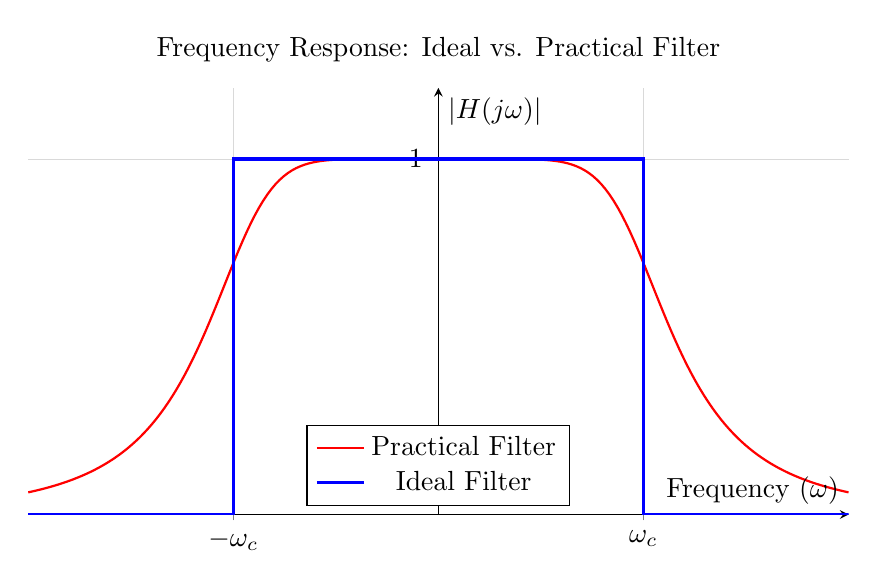
\begin{tikzpicture}
	\begin{axis}[
		width=12cm,
		height=7cm,
		title={Frequency Response: Ideal vs. Practical Filter},
		xlabel={Frequency ($\omega$)},
		ylabel={$|H(j\omega)|$},
		axis lines=middle,
		xmin=-5, xmax=5,
		ymin=0, ymax=1.2,
		xtick={-2.5, 2.5},
		xticklabels={$-\omega_c$, $\omega_c$},
		ytick={1},
		grid=major,
		grid style={line width=.1pt, draw=gray!30},
		legend style={at={(0.5,0.02)}, anchor=south},
		]
		
		% Practical Filter (Butterworth-like magnitude)
		\addplot[red, thick, domain=-5:5, samples=200, mark=none]
		{1/(sqrt(1+(x/2.5)^8))};
		\addlegendentry{Practical Filter};
		
		% Ideal Filter (brick-wall)
		\addplot[blue, very thick, mark=none]
		coordinates {(-5,0) (-2.5,0) (-2.5,1) (2.5,1) (2.5,0) (5,0)};
		\addlegendentry{Ideal Filter};
		
	\end{axis}
\end{tikzpicture}

% --- Second Plot: Impulse Response (Corrected and Refactored) ---
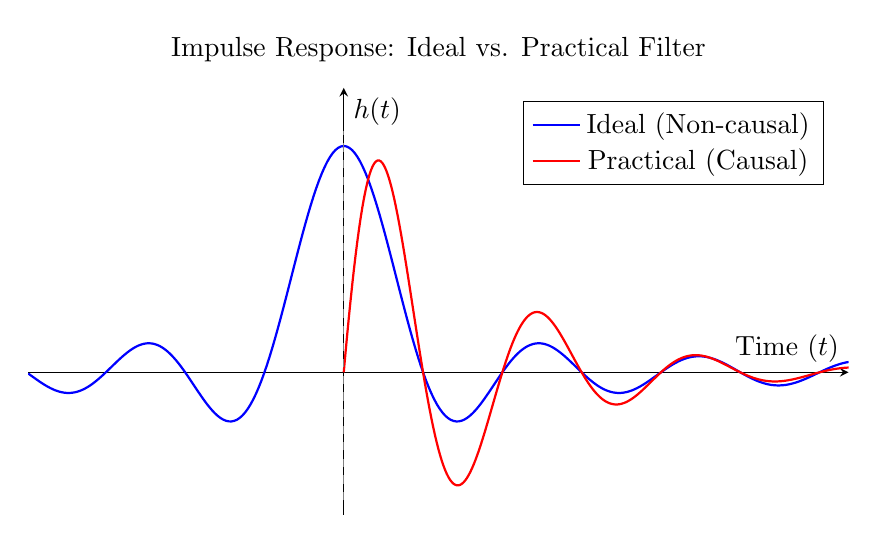
\begin{tikzpicture}
	\begin{axis}[
		width=12cm,
		height=7cm,
		title={Impulse Response: Ideal vs. Practical Filter},
		xlabel={Time ($t$)},
		ylabel={$h(t)$},
		axis lines=middle,
		xmin=-5, xmax=8,
		ymin=-0.5, ymax=1.0,
		xtick={0},
		ytick=\empty,
		grid=major,
		grid style={line width=.1pt, draw=gray!30},
		legend pos=north east,
		% Declare a radian-based sinc function for robustness and clarity.
		% This function computes sin(x)/x, handling the case at x=0.
		declare function={
			sincrad(\x) = (\x==0) ? 1 : sin(\x r)/\x;
		},
		]
		
		% Ideal impulse response is h(t) = (omega_c/pi) * sinc(omega_c*t)
		% With omega_c = 2.5, we plot (2.5/pi) * sincrad(2.5*t)
		\addplot[blue, thick, domain=-5:8, samples=300, mark=none]
		{ (2.5/pi) * sincrad(2.5*x) };
		\addlegendentry{Ideal (Non-causal)};
		
		% Practical impulse response (causal, damped sinusoid)
		\addplot[red, thick, domain=0:8, samples=300, mark=none]
		{exp(-0.5*x)*sin(deg(2.5*x))};
		\addlegendentry{Practical (Causal)};
		
		% Vertical line at t=0 to emphasize causality
		\draw[dashed, gray] (axis cs:0,-0.45) -- (axis cs:0,0.85);
		
	\end{axis}
\end{tikzpicture}









	\caption{Ideal vs. practical filter characteristics.}
	\label{fig:ideal_vs_practical_filter}
\end{figure}

\section*{19.2 Time-Domain Properties of Ideal Filters}

Using the duality property of the Fourier transform, a rectangular spectrum corresponds to a sinc-shaped impulse response:
\[
h(t) = \frac{\sin(\omega_c t)}{\pi t}
\]

This impulse response has two critical problems:
\begin{enumerate}[noitemsep]
	\item \textbf{Non-causality:} The sinc function is non-zero for $t<0$, requiring the system to respond before the input is applied. Therefore, \textbf{ideal filters are not physically realizable} for real-time applications.
	\item \textbf{Infinite Duration:} The impulse response contains oscillations that decay slowly and extend infinitely in time.
\end{enumerate}


\section*{19.3 Non-Ideal, Practical Filters}

Practical filters must approximate ideal behavior.

Non-ideal filters have three frequency regions:
\begin{itemize}[noitemsep]
	\item \textbf{Passband:} Frequencies passed with minimal attenuation, typically allowing small ripple (e.g., within 1\%)
	\item \textbf{Stopband:} Frequencies significantly attenuated, with specified maximum ripple (e.g., less than 0.1\% of passband gain)
	\item \textbf{Transition Band:} The region between passband and stopband where the filter's gain transitions
\end{itemize}

\begin{figure}[H]
	\centering
	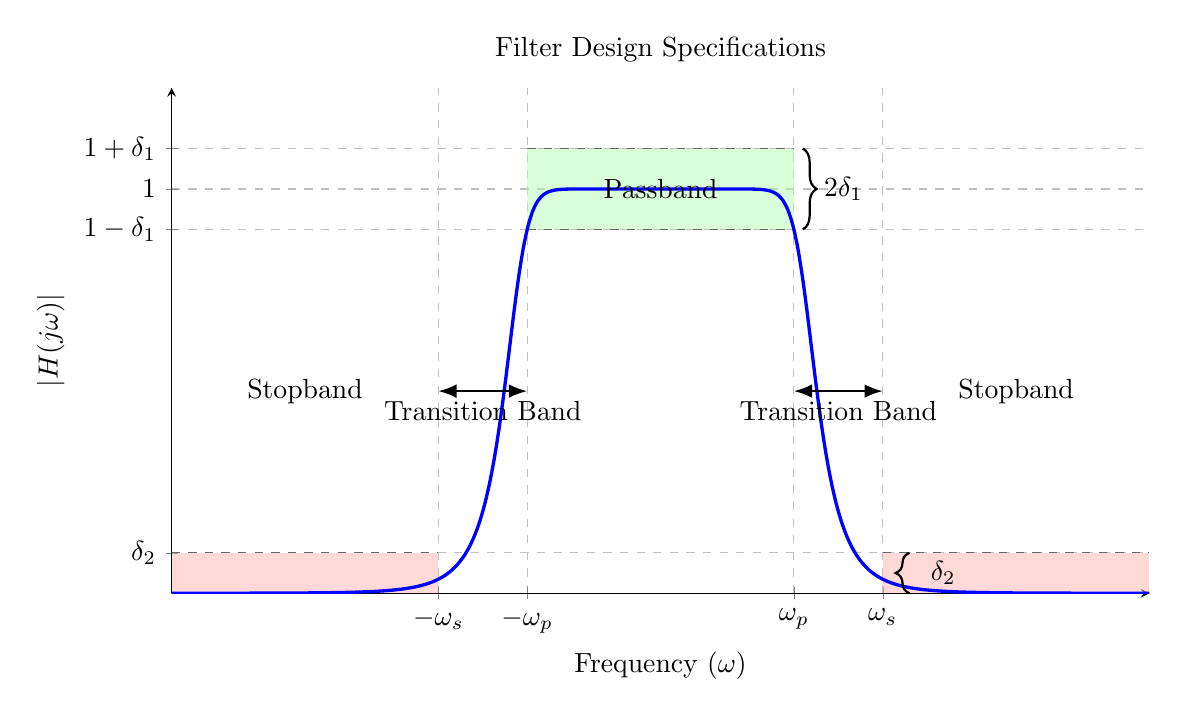
\begin{tikzpicture}
	\begin{axis}[
		width=14cm,
		height=8cm,
		title={Filter Design Specifications},
		xlabel={Frequency ($\omega$)},
		ylabel={$|H(j\omega)|$},
		axis lines=left,
		axis x line=bottom,
		xmin=-5.5, xmax=5.5,
		ymin=0, ymax=1.25,
		xtick={-2.5, -1.5, 1.5, 2.5},
		xticklabels={$-\omega_s$, $-\omega_p$, $\omega_p$, $\omega_s$},
		ytick={0.1, 0.9, 1, 1.1},
		yticklabels={$\delta_2$, $1-\delta_1$, $1$, $1+\delta_1$},
		grid=major,
		grid style={dashed, gray!50},
		no marks,
		xlabel style={at={(ticklabel cs:0.5)},anchor=near ticklabel}, % Center xlabel
		]
		
		% 1. Shade the allowed regions (Pass regions)
		\fill[green!30, opacity=0.5] (axis cs:-1.5, 0.9) rectangle (axis cs:1.5, 1.1);
		\fill[red!30, opacity=0.5] (axis cs:-5.5, 0) rectangle (axis cs:-2.5, 0.1);
		\fill[red!30, opacity=0.5] (axis cs:2.5, 0) rectangle (axis cs:5.5, 0.1);
		

		% 3. Draw tolerance boundary lines
		\draw[dashed, black!60] (axis cs:-5.5, 0.1) -- (axis cs:-2.5, 0.1);
		\draw[dashed, black!60] (axis cs:2.5, 0.1) -- (axis cs:5.5, 0.1);
		\draw[dashed, black!60] (axis cs:-1.5, 0.9) -- (axis cs:1.5, 0.9);
		\draw[dashed, black!60] (axis cs:-1.5, 1.1) -- (axis cs:1.5, 1.1);
		
		% 4. Plot a filter response that MEETS the specifications
		\addplot[blue, very thick, domain=-5.5:5.5, samples=201, smooth] {1/sqrt(1 + 0.2345*(x/1.5)^16)};
		
		% 5. Add annotations and labels
		% Region labels
		\node[align=center] at (axis cs:0, 1.0) {Passband}; % Centered in the allowed region
		\node at (axis cs:-4, 0.5) {Stopband};
		\node at (axis cs:4, 0.5) {Stopband};
		
		% Transition band arrows
		\draw[<->, >=Latex, thick] (axis cs:1.5, 0.5) -- (axis cs:2.5, 0.5)
		node[midway, below] {Transition Band};
		\draw[<->, >=Latex, thick] (axis cs:-2.5, 0.5) -- (axis cs:-1.5, 0.5)
		node[midway, below] {Transition Band};
		
		% Tolerance braces (using 'axis cs' for robust positioning)
		\draw [decorate,decoration={brace,amplitude=5pt,mirror}, thick] 
		(axis cs:1.6, 0.9) -- (axis cs:1.6, 1.1) node [midway, right, xshift=4pt] {$2\delta_1$};
		\draw [decorate,decoration={brace,amplitude=5pt}, thick] 
		(axis cs:2.8, 0) -- (axis cs:2.8, 0.1) node [midway, right, xshift=4pt] {$\delta_2$};
		
	\end{axis}
\end{tikzpicture}









	\caption{Filter frequency regions}
	\label{fig:filter_regions}
\end{figure}

\paragraph{The Fundamental Trade-off:}
A fundamental trade-off exists between frequency-domain and time-domain performance:
\begin{itemize}[noitemsep]
	\item \textbf{Sharper frequency cutoffs} (narrower transition bands) produce \textbf{increased overshoot} in the time domain
	\item \textbf{Wider transition bands} (smoother frequency cutoffs) produce less overshoot in the time domain.
\end{itemize}

\begin{remark}
Interactive filter design tools demonstrate how narrowing the transition band increases step response overshoot.
\end{remark}
\newpage
\section*{19.4 Analog vs. Digital Implementation}

\subsection*{19.4.1 Analog Filter Advantages}
\begin{itemize}[noitemsep]
	\item \textbf{Zero latency:} No computational delay in processing
	\item \textbf{High speed:} Operation at MHz frequencies with simple op-amp circuits
	\item \textbf{Large dynamic range:} Both amplitude (10 million:1) and frequency (seven decades simultaneously)
	\item \textbf{Real-time operation:} Natural parallel processing of all frequency components
\end{itemize}

\subsection*{19.4.2 Digital Filter Advantages}
\begin{itemize}[noitemsep]
	\item \textbf{Precise specifications:} Exact filter coefficients without component tolerances
	\item \textbf{Stability:} Performance independent of temperature and aging
	\item \textbf{Flexibility:} Software-based design enables easy modification
	\item \textbf{Better frequency response:} Better passband flatness and stopband rejection
\end{itemize}

Digital filters exhibit inherent latency due to analog-to-digital conversion and processing delays.

\section*{19.5 The Discrete Fourier Transform (DFT)}

While the DTFT provides a complete frequency-domain representation for discrete-time signals, it is defined for signals of infinite duration and produces a continuous function of frequency. For practical computation, we need a finite-length, discrete-frequency representation: the \textbf{Discrete Fourier Transform (DFT)}.

\subsection*{19.5.1 From DTFT to DFT}

Consider a finite-length sequence $x[n]$ of length $N$ (i.e., $x[n] = 0$ for $n < 0$ and $n \geq N$). The DTFT of this sequence is:
\[
X(e^{j\omega}) = \sum_{n=0}^{N-1} x[n]e^{-j\omega n}
\]

The DFT samples this continuous DTFT at $N$ equally spaced frequencies:
\[
\omega_k = \frac{2\pi k}{N}, \quad k = 0, 1, 2, \ldots, N-1
\]

\begin{definition}
	For a finite-length sequence $x[n]$ of length $N$, the \textbf{Discrete Fourier Transform (DFT)} is:
	\[
	X[k] = \sum_{n=0}^{N-1} x[n]e^{-j\frac{2\pi kn}{N}}, \quad k = 0, 1, 2, \ldots, N-1
	\]
	The \textbf{Inverse DFT (IDFT)} is:
	\[
	x[n] = \frac{1}{N}\sum_{k=0}^{N-1} X[k]e^{j\frac{2\pi kn}{N}}, \quad n = 0, 1, 2, \ldots, N-1
	\]
\end{definition}

\subsection*{19.5.2 Key Properties of the DFT}

\begin{itemize}[noitemsep]
	\item \textbf{Finite Length:} Both time and frequency domains are finite and discrete
	\item \textbf{Periodicity:} The DFT implicitly treats $x[n]$ as one period of a periodic sequence
	\item \textbf{Relationship to DTFT:} $X[k] = X(e^{j\omega})|_{\omega = 2\pi k/N}$ - the DFT samples the DTFT
	\item \textbf{Computational Efficiency:} The Fast Fourier Transform (FFT) algorithm computes the DFT in $O(N \log N)$ operations instead of $O(N^2)$
\end{itemize}

\subsection*{19.5.3 Relationship to DTFS}

The DFT is essentially the same as the Discrete-Time Fourier Series (DTFS) coefficients for a periodic signal. If we view $x[n]$ as one period of a periodic sequence $\tilde{x}[n]$, then:
\[
X[k] = N \cdot a_k
\]
where $a_k$ are the DTFS coefficients of $\tilde{x}[n]$.

\begin{remark}
	The DFT provides a complete, computable representation for finite-length sequences. The FFT algorithm makes DFT computation efficient for large $N$, enabling real-time signal processing applications.
\end{remark}
\section*{Summary and Next Lecture}
	\begin{itemize}[noitemsep]
		\item Ideal filters are non-causal and unrealizable in real-time
		\item Sharp frequency cutoffs produce ringing and overshoot in time domain
		\item Practical filters involve frequency-time domain trade-offs
		\item Analog and digital implementations have distinct advantages
		\item DFT samples the DTFT at discrete frequencies; FFT enables efficient computation
		\item \textbf{Next time:} The sampling theorem and bridging continuous-time and discrete-time signals
	\end{itemize}

\end{document}
